\begin{figure}
  \centering 
  \begin{subfigure}[b]{0.45\textwidth}
    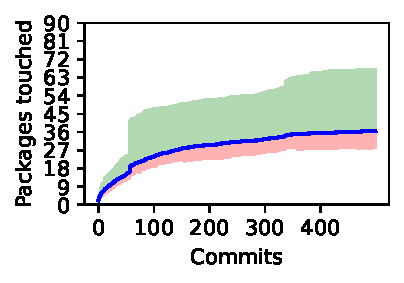
\includegraphics[width=\textwidth]{sections/results/packages/time_series_components_touched.packages.all.founders.commits_500.pdf}
    \caption{Packages for All founders (n=281, $\mu$=1.0, median=1.0 \& std=0.0)}
    \label{figure.sections/results/packages/time_series_components_touched.packages.all.founders.commits_500.pdf}
  \end{subfigure}
  \begin{subfigure}[b]{0.45\textwidth}
    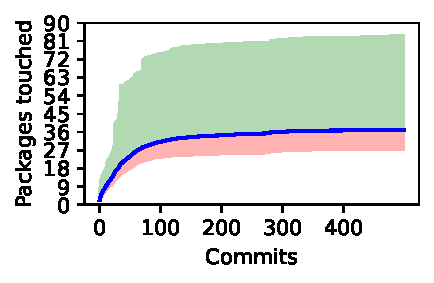
\includegraphics[width=\textwidth]{sections/results/packages/time_series_components_touched.packages.all.joiners.commits_500.pdf}
    \caption{Packages for All joiners (n=16138, $\mu$=1.0, median=1.0 \& std=0.0)}
    \label{figure.sections/results/packages/time_series_components_touched.packages.all.joiners.commits_500.pdf}
  \end{subfigure}
\newpage 
\vspace{3mm}
  \begin{subfigure}[b]{0.45\textwidth}
    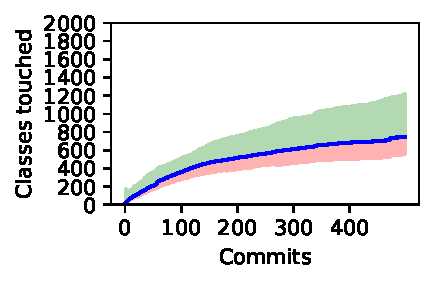
\includegraphics[width=\textwidth]{sections/results/classes/time_series_components_touched.classes.all.founders.commits_500.pdf}
    \caption{Classes for All founders (n=281, $\mu$=1.0, median=1.0 \& std=0.0)}
    \label{figure.sections/results/classes/time_series_components_touched.classes.all.founders.commits_500.pdf}
  \end{subfigure}
  \begin{subfigure}[b]{0.45\textwidth}
    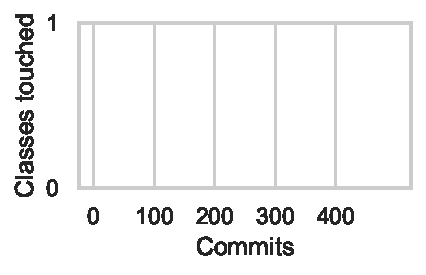
\includegraphics[width=\textwidth]{sections/results/classes/time_series_components_touched.classes.all.joiners.commits_500.pdf}
    \caption{Classes for All joiners (n=16138, $\mu$=1.0, median=1.0 \& std=0.0)}
    \label{figure.sections/results/classes/time_series_components_touched.classes.all.joiners.commits_500.pdf}
  \end{subfigure}
\newpage 
  \begin{subfigure}[b]{0.45\textwidth}
    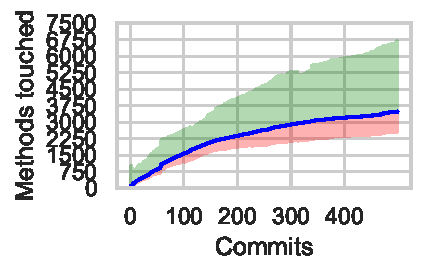
\includegraphics[width=\textwidth]{sections/results/methods/time_series_components_touched.methods.all.founders.commits_500.pdf}
    \caption{Methods for All founders (n=281, $\mu$=1.0, median=1.0 \& std=0.0)}
    \label{figure.sections/results/methods/time_series_components_touched.methods.all.founders.commits_500.pdf}
  \end{subfigure}
  \begin{subfigure}[b]{0.45\textwidth}
    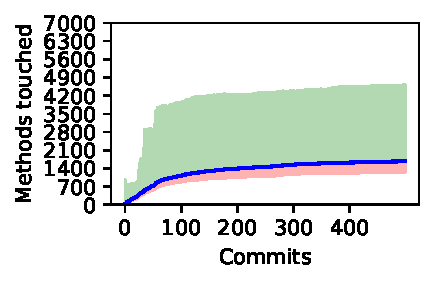
\includegraphics[width=\textwidth]{sections/results/methods/time_series_components_touched.methods.all.joiners.commits_500.pdf}
    \caption{Methods for All joiners (n=16138, $\mu$=1.0, median=1.0 \& std=0.0)}
    \label{figure.sections/results/methods/time_series_components_touched.methods.all.joiners.commits_500.pdf}
  \end{subfigure}
\caption{A time series for the all commits, excluding transient, with the average mean (blue line), all components touched (y-axis) against the number of commits (x-axis) for six (6) developer categories. Green is the standard deviation above the mean, and pink is the standard deviation below the mean.}\end{figure}
\clearpage 
\newpage 
